O motor de passo híbrido pode ser analisado através do modelo dinâmico de acordo com a Fig. \ref{fig:fig1} por apresentar respostas das características em regime transitório e estacionário. O circuito equivalente é construído supondo que o circuito magnético é linear (não saturado) e a indutância mútua entre as fases é desconsiderada.

\begin{figure}[H]
	\centering
	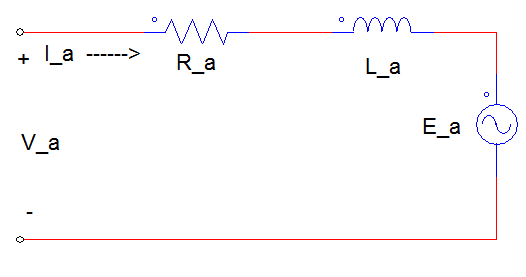
\includegraphics[width = .8\columnwidth]{Images/graficofasea.PNG}
	\caption{ Circuito equivalente da bobina A.}
	\label{fig:fig1}
\end{figure}

No modelo, $R_a$ e $L_a(\theta)$ representa respectivamente a resistência e a indutância da fase A do enrolamento. O enrolamento varia a indutância em função da posição do rotor.

\begin{eqnarray}
	\label{eq:eq1a}
	L_a(\theta) = L_0 + L_1\cos(\rho \theta)
\end{eqnarray}

Onde:

\begin{itemize}
	 \item $L_0$ - indutância média,
	 \item $L_1$ - indutância variável,
	 \item $\rho$ - número de dentes do rotor.
\end{itemize}


Note que a posição de referência ($\theta = 0$), é quando o dente do rotor está completamente alinhado com o polo do eixo A, então o enrolamento da fase A terá a indutância máxima ($L_1^{max}$).

Este modelo $R_a$ e $L_a$ representa respectivamente a resistência e indutância da fase A. Devido ao tamanho do entreferro, a indução dos enrolamentos do motor de passo híbrido pode ser considerado independente da posição do rotor. 

No caso de um motor de duas fases a tensão $E_a$ representa a FEM induzida na bobina A, conforme \cite{Acarnley}. Sendo uma função senoidal da posição do rotor

\begin{eqnarray}
	\label{eq:eq2a}
	E_a = \omega \rho \psi_m \sin(\rho \theta)
\end{eqnarray}

similar a FEM induzida pela bobina B, que é dado por:

\begin{eqnarray}
		\label{eq:eq3a}
		E_b = \omega \rho \psi_m \sin(\rho \theta - \lambda)
\end{eqnarray}

onde:

\begin{itemize}
	\item $\rho$ - número de dentes do rotor,
	\item $\psi_m$ - máximo fluxo concatenado, 	\item $\theta$ - posição angular do rotor,
	\item $\lambda$ - angulo de fase.
\end{itemize}

No caso de duas fases do estator, $\lambda = \frac{\pi}{2}$ e a equação de $E_b$ é modificado como se segue a equação (\ref{eq:eq4a}).

\begin{eqnarray}
		\label{eq:eq4a}
		E_b = \omega \rho \psi_m \cos(\rho \theta )
\end{eqnarray}

De acordo com a análise da Fig. \ref{fig:fig1} e as Equações (\ref{eq:eq1a}), (\ref{eq:eq2a}) e (\ref{eq:eq4a}), as equações das correntes são apresentadas conforme \cite{kenjo}.

\begin{eqnarray}
	\label{eq:eq5a}
	\frac{d i_A(t)}{dt} = \frac{1}{L_a}\left(V_A - Ri_A(t) + \omega(t) \rho \psi_m \sin(\rho \theta) \right) \\
	\label{eq:eq5b}
	\frac{d i_B(t)}{dt} = \frac{1}{L_b}\left(V_B - Ri_B(t) - \omega(t) \rho \psi_m \cos(\rho \theta) \right) 
\end{eqnarray}

Onde:

\begin{itemize}
	\item $V_A, V_B$ - tensões de fase,
	\item $R$ - resistência de fase do enrolamento,
	\item $i_A,\ i_B$ - correntes de fase.
\end{itemize}

O torque eletromagnético ($T_e$) é formado pelas componentes do torque gerado referente a cada fase como segue nas equações (\ref{eq:eq6a}), (\ref{eq:eq6b}) \cite{stepersimulink}.

\begin{eqnarray}
\label{eq:eq6a}
T_A = i_A \rho \psi_m \sin(\rho \theta)\\
\label{eq:eq6b}
T_B = i_B \rho \psi_m \cos(\rho \theta) 
\end{eqnarray}

Se o estator e o rotor tem dentes, o torque eletromagnético é complementado pela componente de torque devido a relutância gerado pela saliências do endentamento, chamado de torque de retenção (\textit{detent torque}) ou torque endentação ($T_d$), possui a equação (\ref{eq:eq7a}) \cite{kenjo}.

\begin{eqnarray}
\label{eq:eq7a}
T_d = T_{d}^{max}\sin(2 \rho \theta)
\end{eqnarray}

O torque eletromagnético produzido por motor de passo híbrido de duas fases é igual ao somatório resultante da interação entre as correntes das duas fases além do fluxo magnético formado pelos ímãs juntamente com o torque de endentação como demonstra a equação (\ref{eq:eq8a}) \cite{mathworkmotor}.

\begin{eqnarray}
	\label{eq:eq8a}
	T_e = - \rho \psi_m i_A \sin(\rho \theta) - \rho \psi_m i_B \cos(\rho \theta ) - T_d
\end{eqnarray}

O movimento do rotor é descrito pela equação (\ref{eq:eq9a})de rotação do movimento, o que leva em conta a soma da inércia, torque de carga, torque eletromagnético e o torque de atrito viscoso ($T_L$)\cite{stepersimulink} .

\begin{eqnarray}
\label{eq:eq9a}
\frac{d\omega(t)}{dt} = T_e(t) - T_L - B\omega(t)
\end{eqnarray}

Substituindo a equação \ref{eq:eq8a} em \ref{eq:eq9a} obtemos a equação \ref{eq:eq10a}.

%\scriptsize
% Nao adianta diminuir o tamanho, nao fica centralizado, e ainda por cima fica ruim pra ler, deixa normal mesmo

\begin{eqnarray}
\label{eq:eq10a}
j\frac{d\omega(t)}{dt} = - \rho \psi_m i_A \sin(\rho \theta) - \rho \psi_m i_B \cos(\rho \theta ) )-\\ \nonumber T_{d}^{max}\sin(2 \rho \theta)  - T_L - B\omega(t)
\end{eqnarray}


Com as equações definidas, utiliza-se o modelo de espaço de estados para a resolução em tempo contínuo dadas as devidas considerações expostas anteriormente. 

\subsection{Simulação Computacional}

É possível simular o comportamento do motor por modelo genérico utilizando o $Simulink^\circledR$ conforme apresentado na Fig. \ref{fig:fig2}.

\begin{figure}[!h]
	\centering
	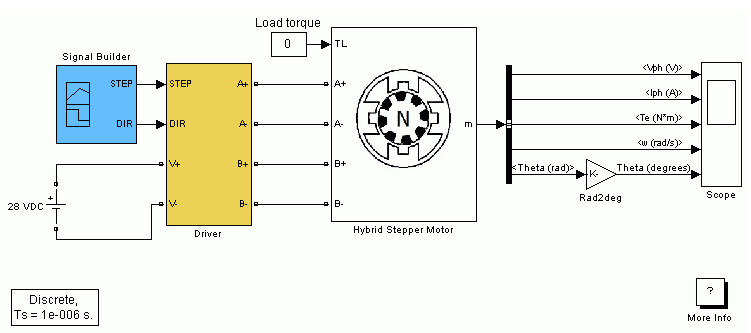
\includegraphics[width= \columnwidth]{Images/modeloEE_HSM.PNG}
	\caption{ Modelo Genérico do Motor de Passo Híbrido - $Simulink^{\circledR}$ \cite{mathworkmotor} }
	\label{fig:fig2}
\end{figure}

O bloco representando o motor oferece 5 sinais de saída sendo eles:

\begin{itemize}
	\item Tensão de fase ($V_f$);
	\item Corrente de fase ($I_f$);
	\item Torque eletromagnético ($T_e$);
	\item Velocidade angular do rotor ($\omega$);
	\item Posição do rotor ($\theta$).
\end{itemize}

Os parâmetros usados no modelo de motor de passo são usualmente obtidos na folha de dados do fabricante. No caso onde os parâmetros não estão disponíveis, pode ser determinado através de medidas experimentais.

Os parâmetros encontrados na folha de dados são geralmente: números de fases, torque de rotor travado (\textit{holding torque}), angulo de passo, tensão de fase, resistência do enrolamento($R_a$), máxima indutância($L_1^{max},\ para\ \theta=0$), indutância média ($L_0$) e inércia do motor ($J$).

O máximo torque de retenção($T_d^{max}$) não é especificado. Este parâmetro pode  ser considerado entre $1\%-10\%$ do torque máximo de rotor travado. O máximo fluxo concatenado ($\psi_m$) não é sempre especificado. Este parâmetro pode ser obtido de forma experimental pelo acionamento do motor a uma velocidade constante $N$ (rpm) e medindo em circuito aberto a máxima tensão de enrolamento $E_f$ (V).


O parâmetro $\psi_m$ é computacionalmente obtido pela equação (\ref{eq:eq11a}) \cite{mathworkmotor}.

\begin{eqnarray}
\label{eq:eq11a}
\psi_m = \left(\frac{30}{P \pi}\right) \left(\frac{E_f}{N}\right)
\end{eqnarray}

Onde:

\begin{itemize}
	\item $P$ - número de pares de pólos dado por $P = \frac{360}{2mpasso}$. Aqui $m$= número de fases , $passo$ = ângulo do passo em graus.
\end{itemize}

\subsection{Curva de Torque $vs$ Velocidade \cite{motorbas}}
A característica de torque versus velocidade é chave para selecionar adequadamente o motor, método de acionamento para uma aplicação específica. Esta características são dependente do motor, do modo de excitação e do tipo de driver ou método de acionamento. Para melhor entender a curva é útil definirmos os diferentes aspectos da curva representado na Fig. \ref{fig:fig3}.

\begin{figure}[H]
	\centering
	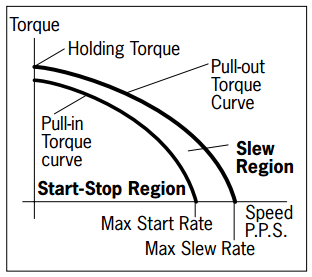
\includegraphics[scale=.6]{Images/curvatorquevelocidade_HSM.PNG}
	\caption{ Curva ideal de Torque \textit{versus} Velocidade do motor de passo }
	\label{fig:fig3}
\end{figure}

Torque de arranque (\textit{holding torque}), é o máximo torque produzido quando o motor está parado.

Curva de Carga (\textit{pull-out curve}) define uma área referido como região de operação (\textit{slew region}). Esta curva fornece a frequência máxima com que o motor pode operar sem perder o sincronismo. O motor deve operar dentro desta região (\textit{slew region}) para seu correto funcionamento 

Máxima frequência de operação (\textit{maximum slew rate}), é a máxima frequência de operação do motor sem carga aplicada.

As características da curva de carga (\textit{pull-out curve}) varia também de acordo com a carga. Quanto maior a inércia da carga, menor será a área da curva de partida. Podemos ver a partir do formato da curva que a velocidade afeta a capacidade de torque de saída, diminuindo a medida que a velocidade aumenta. Isto ocorre pois em altas velocidades o circuito tem caráter predominantemente indutivo.


